\chapter{Resultados}
\label{chap:resultados}

Neste capítulo, com base na solução proposta, serão apresentados alguns resultados obtidos a partir de diferentes conjuntos de regras. Logo após, serão avaliados dados estatísticos de cada um dos modelos gerados. Tais resultados foram obtidos por meio da utilização de um \textit{notebook} com processador Intel Core i5, 2.20GHz, 8GB de memória RAM, sistema operacional Linux Mint 20 Cinnamon, arquitetura de 64 bits e placa de vídeo Intel Corporation HD Graphics 5500. Por fim, também serão apresentadas algumas restrições encontradas.

\section{Modelos gerados}
\label{sec:resultados_modelos}

O primeiro resultado a ser apresentado baseia-se no edifício da Figura \ref{fig:selex_limitation}, o qual, segundo \citeonline{wonka2018}, ainda representa um desafio de modelagem para a \gls{SELEX}. As regras a seguir representam cada uma das etapas de geração. Posteriormente, na Figura \ref{fig:modelo_final_solucao}, são mostrados os modelos resultantes de cada operação, bem como a árvore de formas final.

Inicialmente, são definidas as características do modelo por meio da regra:

\vspace{0.3cm}

\begin{enumerate}
    \item[] \textit{\#C1: Initial settings} \\
            \qquad \textit{label = "building"; width = 9; depth = 8; height = 5;} 
\end{enumerate}

\vspace{0.3cm}

Logo após, o processo continua a partir das seguintes regras:

\vspace{0.3cm}

\begin{enumerate}[label=(\alph*)]
    \item \textit{\#C2: Generating mass model} \\
            \textit{\{<> $-$> createShape(label, width, depth, height)\};}
            
    \item \textit{\#C3: Adding virtual shape} \\
            \qquad \textit{\{<descendant()[label=="building"]/[label=="building\_front"]>} \\
            \qquad \textit{$-$> createGrid("main\_front\_grid", 3, 6)\};}
    
    \item \textit{\#C4: Selecting left region and performing extrusion} \\
            \qquad \textit{\{<descendant()[label=="building"]/[label=="building\_front"]/} \\
            \qquad \textit{[label=="main\_front\_grid"]/[type=="cell"]} \\
            \qquad \textit{[rowIdx in (1, 2, 3)] [colIdx in (1, 2)] [::groupRegions()]>} \\
            \qquad \textit{$-$> addVolume("fac\_1", "building\_front", 2.5,} \\
            \qquad \textit{["fac\_1\_front", "fac\_1\_left", "fac\_1\_right"])\};}
            
    \item \textit{\#C5: Applying roundShape deformation} \\
            \qquad \textit{\{<descendant()[label=="building"]/[label=="building\_front"]/} \\
            \qquad \textit{[label=="fac\_1"]/[label=="fac\_1\_front"]>} \\
            \qquad \textit{$-$> roundShape("front", "outside", 0.33, 30, "main\_front", "vertical")\};}
            
    \item \textit{\#C6: Selecting middle region and performing extrusion} \\
            \qquad \textit{\{<descendant()[label=="building"]/[label=="building\_front"]/} \\
            \qquad \textit{[label=="main\_front\_grid"]/[type=="cell"]} \\
            \qquad \textit{[rowIdx in (1, 2, 3)] [colIdx in (3, 4)] [::groupRegions()]>} \\
            \qquad \textit{$-$> addVolume("fac\_2", "building\_front", 3,} \\
            \qquad \textit{["fac\_2\_front", "fac\_2\_left", "fac\_2\_right"])\};}
            
    \item \textit{\#C7: Applying roundShape deformation} \\
            \qquad \textit{\{<descendant()[label=="building"]/[label=="building\_front"]/} \\
            \qquad \textit{[label=="fac\_2"]/[label=="fac\_2\_front"]>} \\
            \qquad \textit{$-$> roundShape("front", "outside", 0.33, 30, "main\_front", "vertical")\};}
    
    \item \textit{\#C8: Selecting bottom-right region and performing extrusion} \\
            \qquad \textit{\{<descendant()[label=="building"]/[label=="building\_front"]/} \\
            \qquad \textit{[label=="main\_front\_grid"]/[type=="cell"]} \\
            \qquad \textit{[rowIdx in (2, 3)] [colIdx in (5, 6)] [::groupRegions()]>} \\
            \qquad \textit{$-$> addVolume("fac\_3", "building\_front", 3.5,} \\
            \qquad \textit{["fac\_3\_front", "fac\_3\_left", "fac\_3\_right"])\};}
            
    \item \textit{\#C9: Applying roundShape deformation} \\
            \qquad \textit{\{<descendant()[label=="building"]/[label=="building\_front"]/} \\
            \qquad \textit{[label=="fac\_3"]/[label=="fac\_3\_front"]>} \\
            \qquad \textit{$-$> roundShape("front", "outside", 0.33, 30, "main\_front", "vertical")\};}
            
    \item \textit{\#C10: Selecting top-right region and performing extrusion} \\
            \qquad \textit{\{<descendant()[label=="building"]/[label=="building\_front"]/} \\
            \qquad \textit{[label=="main\_front\_grid"]/[type=="cell"]} \\
            \qquad \textit{[rowIdx in (1)] [colIdx in (5, 6)] [::groupRegions()]>} \\
            \qquad \textit{$-$> addVolume("fac\_4", "building\_front", 2,} \\
            \qquad \textit{["fac\_4\_front", "fac\_4\_left", "fac\_4\_right"])\};}
    
    \item \textit{\#C11: Applying roundShape deformation} \\
            \qquad \textit{\{<descendant()[label=="building"]/[label=="building\_front"]/} \\
            \qquad \textit{\{<descendant()[label=="building"]/[label=="building\_front"]/} \\
            \qquad \textit{[label=="fac\_4"]/[label=="fac\_4\_front"]>} \\
            \qquad \textit{$-$> roundShape("front", "outside", 0.33, 30, "main\_front", "vertical")\};}
\end{enumerate}

\vspace{0.3cm}

\begin{figure}[h!]
	\centering
	\captionsetup{width=15cm}
	\Caption{\label{fig:modelo_final_solucao} Modelo de massa do edifício da Figura \ref{fig:selex_limitation}.}	
	\UFCfig{}{
		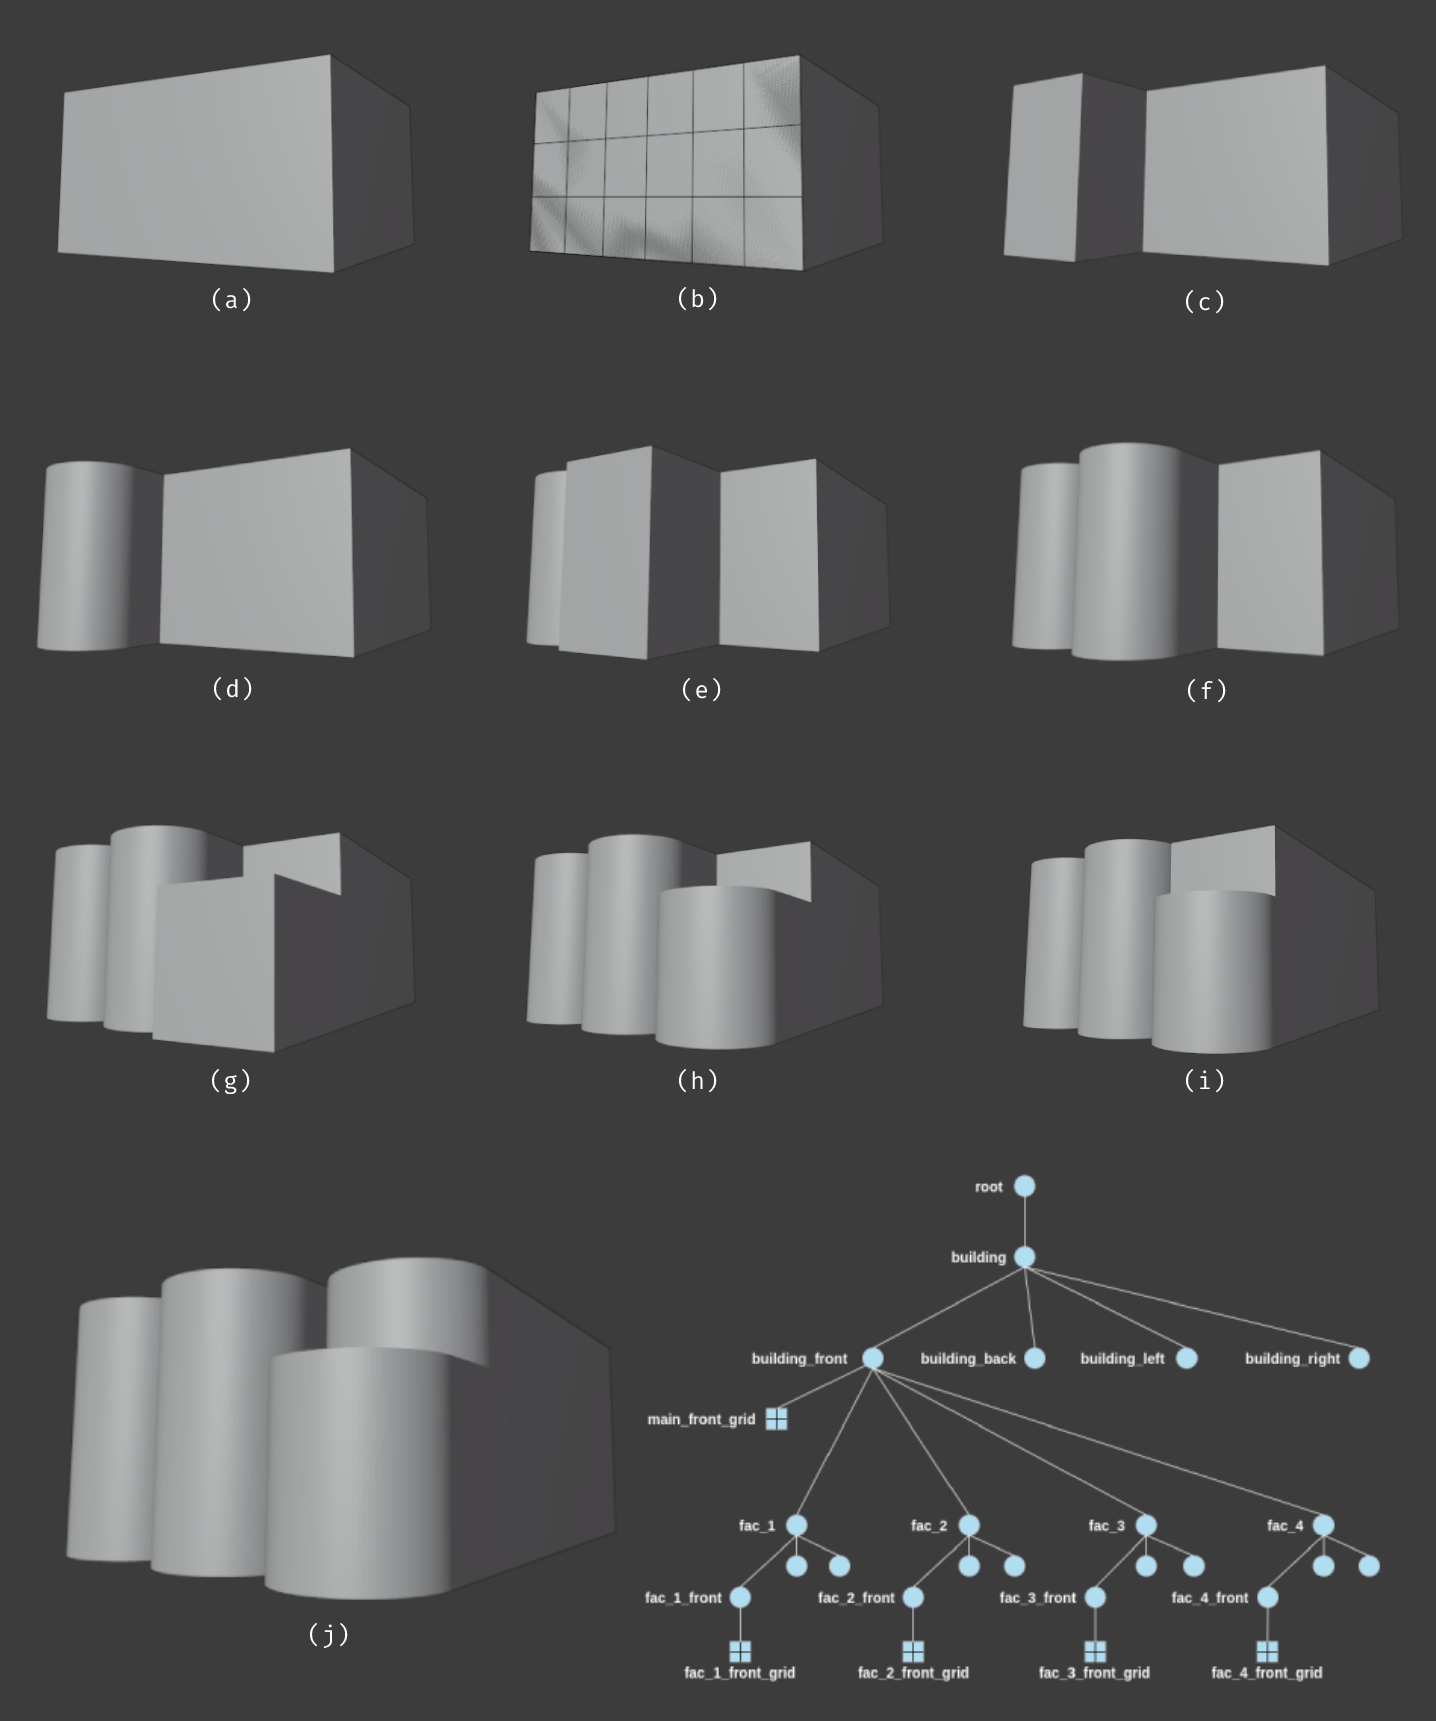
\includegraphics[width=15cm]{figuras/solucao_limitacao.png}
	}
	{\Fonte{Próprio autor}}	
\end{figure}

Na sequência, serão apresentados outros exemplos que exploram diferentes combinações de parâmetros. As regras utilizadas na geração destes modelos encontram-se no Anexo \ref{an:ex_anexo_a}, bem como em um repositório no GitHub \footnote{\href{https://github.com/DanielBrito/monografia/tree/main/Resultados}{https://github.com/DanielBrito/monografia/tree/main/Resultados}}, para uma eventual consulta.

A Figura \ref{fig:resultado_2} representa uma variação do modelo final obtido na Figura \ref{fig:modelo_final_solucao}(j), por meio da inclusão de estruturas arredondadas na região lateral direita.

\begin{figure}[h!]
	\centering
	\captionsetup{width=15cm}
	\Caption{\label{fig:resultado_2} Variação do modelo da Figura \ref{fig:modelo_final_solucao}(j), com modificação na área e lateral.}	
	\UFCfig{}{
		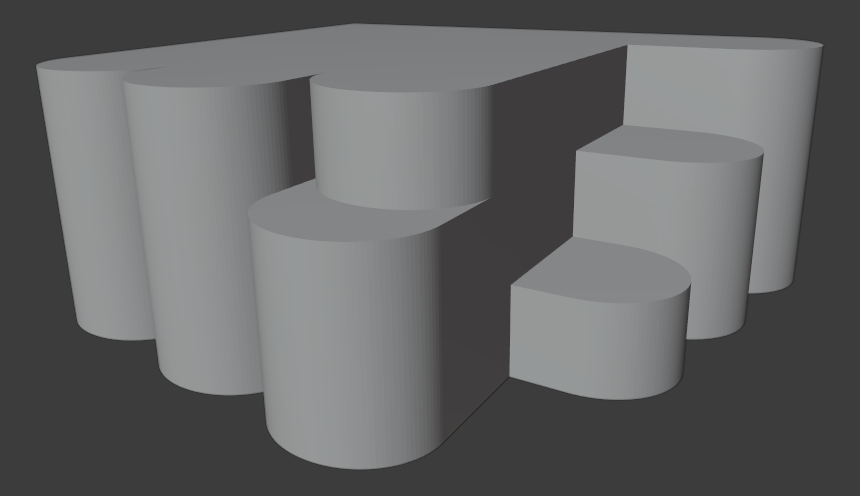
\includegraphics[width=14cm]{figuras/resultado_2.png}
	}
	{\Fonte{Próprio autor}}	
\end{figure}

A Figura \ref{fig:resultado_3}(a), por sua vez, representa uma variação do modelo apresentado por \citeonline{wonka2018}, conforme ilustrado na Figura \ref{fig:exemplo_selex}(o).

\begin{figure}[h!]
	\centering
	\captionsetup{width=15cm}
	\Caption{\label{fig:resultado_3} Variação do modelo apresentado na Figura \ref{fig:exemplo_selex}(o).}
	\UFCfig{}{
		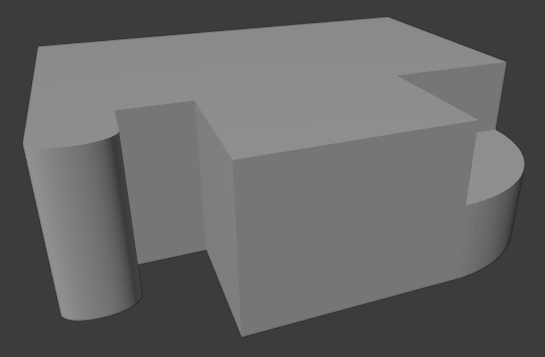
\includegraphics[width=14cm]{figuras/resultado_3.png}
	}
	{\Fonte{Próprio autor}}	
\end{figure}

\newpage

Os modelos apresentados nas Figuras \ref{fig:variacoes_wonka2018}(a), \ref{fig:variacoes_wonka2018}(b), \ref{fig:variacoes_wonka2018}(c) e \ref{fig:variacoes_wonka2018}(d), representam variações dos resultados obtidos por \citeonline{wonka2018}.

\begin{figure}[h!]
	\centering
	\captionsetup{width=15cm}
	\Caption{\label{fig:variacoes_wonka2018} À esquerda, variações dos resultados obtidos por \citeonline{wonka2018}, à direita.}	
	\UFCfig{}{
		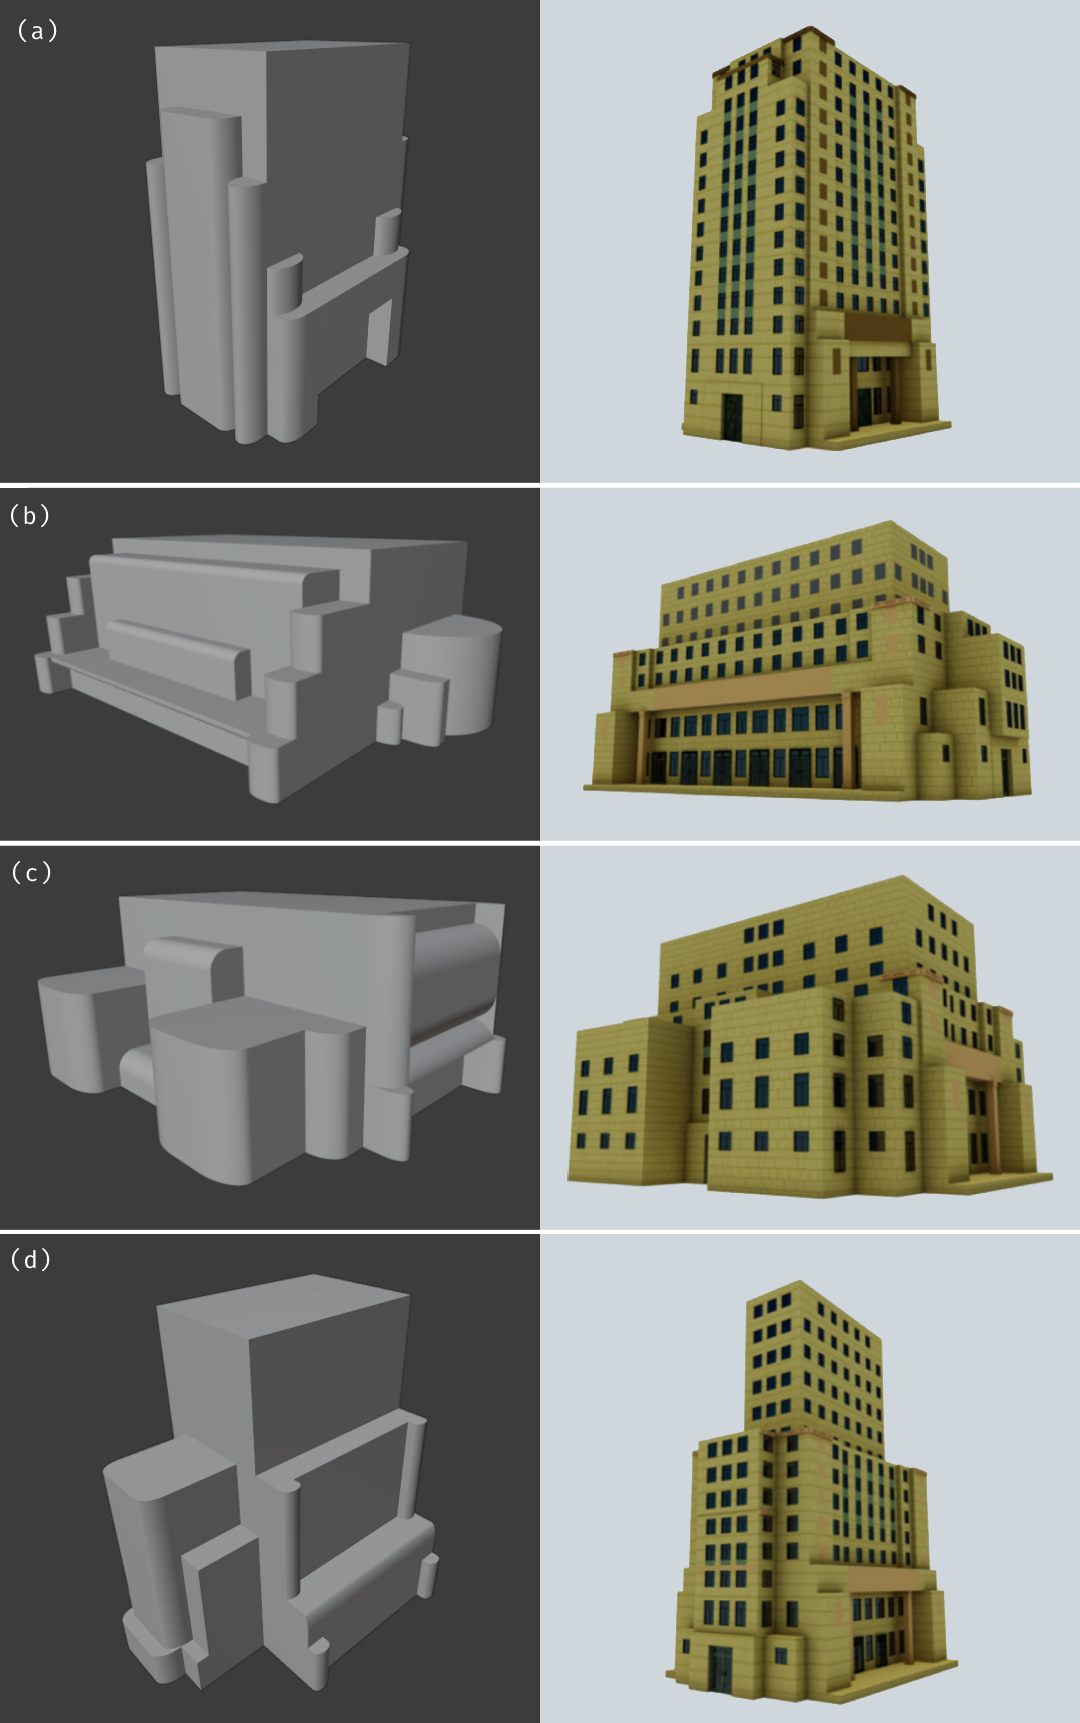
\includegraphics[width=13cm]{figuras/resultados_jiang.png}
	}
	{\Fonte{Próprio autor e \citeonline{wonka2018}}}	
\end{figure}

\newpage

A Figura \ref{fig:resultado_lowpoly} ilustra um dos diferenciais da solução proposta, que é a geração de modelos no formato \textit{low poly}, ou seja, com poucos polígonos, os quais podem ser utilizados em situações que um alto grau de realismo não é requerido.

\begin{figure}[h!]
	\centering
	\captionsetup{width=15cm}
	\Caption{\label{fig:resultado_lowpoly} Variações \textit{low poly} (a) e (b) dos modelos apresentados, respectivamente, na Figura \ref{fig:modelo_final_solucao}(j) e na Figura \ref{fig:vimont}.}
	\UFCfig{}{
		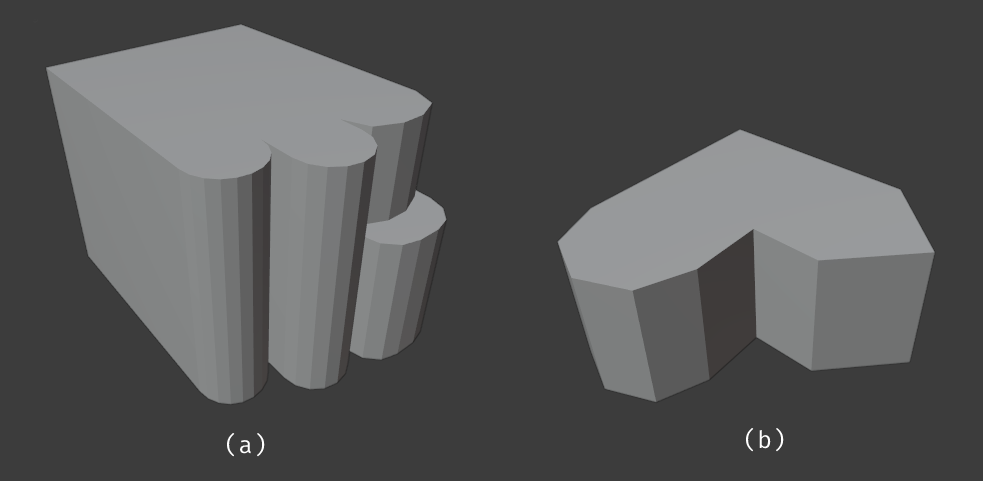
\includegraphics[width=15cm]{figuras/resultado_low_poly.png}
	}
	{\Fonte{Próprio autor}}	
\end{figure}

O modelo da Figura \ref{fig:resultado_9} ilustra o resultado da operação \texttt{roundShape} na região superior, em diferentes faces.

\begin{figure}[h!]
	\centering
	\captionsetup{width=15cm}
	\Caption{\label{fig:resultado_9} Exemplo de arredondamento superior em múltiplas faces.}
	\UFCfig{}{
		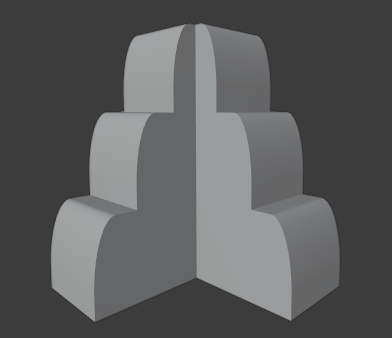
\includegraphics[width=10cm]{figuras/resultado_9.png}
	}
	{\Fonte{Próprio autor}}	
\end{figure}

\newpage

A Figura \ref{fig:resultado_10} demonstra o resultado da geração de um modelo obtido através da combinação de arredondamento externo e interno, produzindo uma arquitetura ondulada.

\begin{figure}[h!]
	\centering
	\captionsetup{width=15cm}
	\Caption{\label{fig:resultado_10} Modelo combinando arredondamento externo e interno.}
	\UFCfig{}{
		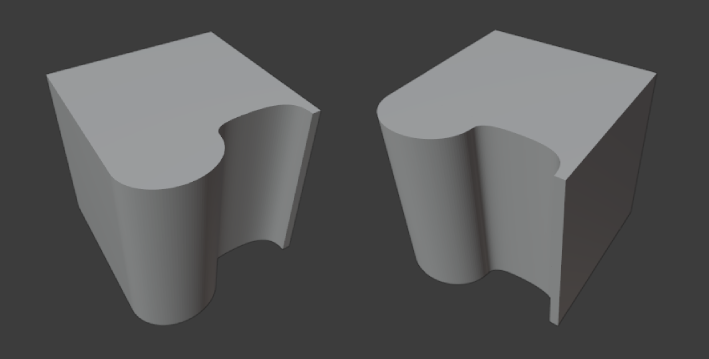
\includegraphics[width=15cm]{figuras/resultado_10.png}
	}
	{\Fonte{Próprio autor}}	
\end{figure}

Nas Figuras \ref{fig:resultado_12} e \ref{fig:resultado_14}, são ilustradas variações dos modelos apresentados por \citeonline{schwarz2015} e \citeonline{wonka2003}, respectivamente.

\begin{figure}[h!]
	\centering
	\captionsetup{width=15cm}
	\Caption{\label{fig:resultado_12} Variação de modelo obtido através da \textit{CGA++}.}
	\UFCfig{}{
		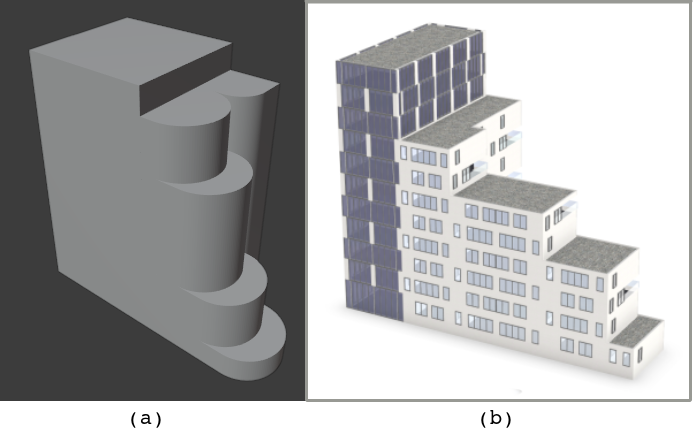
\includegraphics[width=15cm]{figuras/resultado_12.png}
	}
	{\Fonte{(a) Próprio autor e (b) adaptado de \citeonline{schwarz2015}}}	
\end{figure}

\begin{figure}[h!]
	\centering
	\captionsetup{width=15cm}
	\Caption{\label{fig:resultado_14} Variação de modelo obtido através de \textit{split grammar}.}
	\UFCfig{}{
		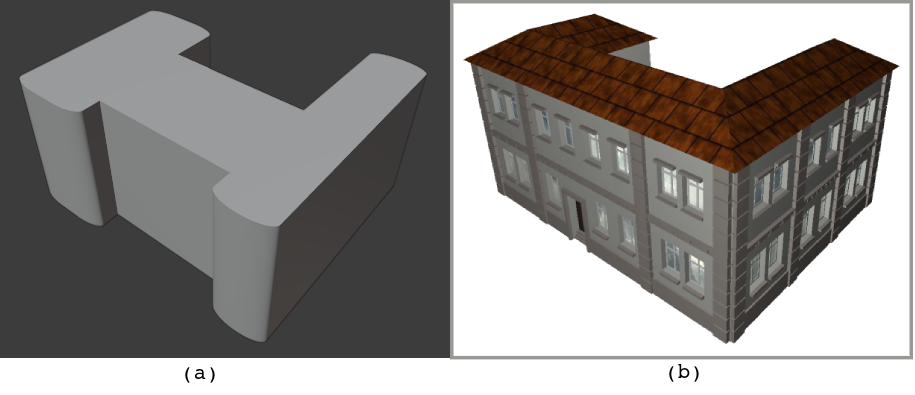
\includegraphics[width=15cm]{figuras/resultado_14.png}
	}
	{\Fonte{(a) Próprio autor e (b) \citeonline{wonka2003}}}	
\end{figure}

\newpage

Por fim, a Figura \ref{fig:resultado_15} ilustra modelos de massa mais complexos, que podem ser obtidos através de uma grande variedade de regras e parâmetros.

\begin{figure}[h!]
	\centering
	\captionsetup{width=15cm}
	\Caption{\label{fig:resultado_15} Modelos com múltiplas variações de arredondamento (a) externo e (b) interno.}
	\UFCfig{}{
		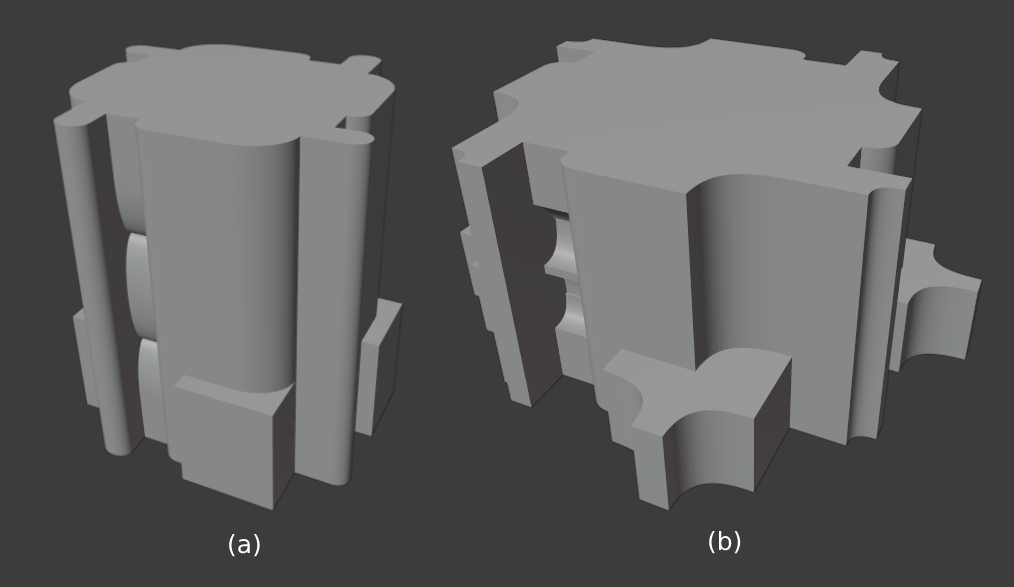
\includegraphics[width=15cm]{figuras/resultados_experimentais.png}
	}
	{\Fonte{Próprio autor}}	
\end{figure}

Uma vez que a capacidade de modelagem da solução proposta foi demonstrada, através de exemplos ilustrativos originais e de variações baseadas nos trabalhos descritos no Capítulo \ref{cap:fundamentacao-teorica}, nas próximas seções, serão apresentados dados estatísticos acerca dos modelos gerados, bem como algumas limitações identificadas.

\newpage

\section{Desempenho}
\label{sec:desempenho}

As técnicas apresentadas nos Capítulos \ref{cap:fundamentacao-teorica} e \ref{cap:trabalhos-correlatos} são aplicadas em diversos cenários, possuindo métricas de desempenho distintas entre si. Portanto, como o presente trabalho é pioneiro na geração procedural de modelos arquiteturais com geometria arredondada utilizando \textit{Selection Expressions}, ainda não existem parâmetros de comparação que estimem a sua qualidade. Logo, a Tabela \ref{tab:dados_estatisticos} apresenta apenas informações estatísticas obtidas a partir dos modelos gerados pela solução proposta, mas que poderão servir como base em trabalhos futuros. Neste caso, não houve uma diferença perceptível no tempo necessário para gerar cada modelo, assim, ele foi descartado.

\begin{table}[!h]
    \centering
    \captionsetup{width=15cm}
    	\Caption{\label{tab:dados_estatisticos} Dados estatísticos dos modelos gerados pela solução proposta.\\}
    \hspace{-1cm}
    \begin{tabular}{|c|c|c|c|c|c|}
        \hline
        \textbf{Figura} & \textbf{Regras} & \textbf{Vértices} & \textbf{Arestas} & \textbf{Faces} & \textbf{Tamanho (MB)} \\ \hline
        \ref{fig:modelo_final_solucao}(f) & 11               & 520               & 780                & 270                & 1,0     \\ \hline
        \ref{fig:resultado_2} & 18               & 904               & 1356                & 468                & 1,1     \\ \hline
        \ref{fig:resultado_3} & 8               & 212               & 319                & 114                & 1,0     \\ \hline
        \ref{fig:variacoes_wonka2018}(a) & 36               & 1576               & 2364                & 822                & 1,3     \\ \hline
        \ref{fig:variacoes_wonka2018}(b) & 31               & 1380               & 2070                & 720                & 1,3     \\ \hline
        \ref{fig:variacoes_wonka2018}(c) & 26               & 1056               & 1584                & 552                & 1,3     \\ \hline
        \ref{fig:variacoes_wonka2018}(d) & 24               & 892               & 1338                & 474                & 1,3     \\ \hline
        \ref{fig:resultado_lowpoly}(a) & 11               & 96               & 144                & 58                & 1,1     \\ \hline
        \ref{fig:resultado_lowpoly}(b) & 8               & 36               & 54                & 24                & 1,0     \\ \hline
        \ref{fig:resultado_9} & 30               & 824               & 1236                & 438                & 1,2     \\ \hline
        \ref{fig:resultado_10} & 9               & 272               & 408                & 144                & 1,1     \\ \hline
        \ref{fig:resultado_12}(a) & 13               & 588               & 882                & 306                & 1,1     \\ \hline
        \ref{fig:resultado_14}(a) & 12               & 520               & 780                & 270                & 1,1     \\ \hline
        \ref{fig:resultado_15}(a) & 58               & 2392               & 3588                & 1254                & 1,5     \\ \hline
        \ref{fig:resultado_15}(b) & 62               & 2152               & 3228                & 1134                & 1,5     \\ \hline
    \end{tabular}
\end{table}

\section{Restrições}
\label{sec:limitacoes}

O presente trabalho representa um avanço no que se refere à geração procedural de modelos arquiteturais com geometria arredondada. Contudo, no decorrer do seu desenvolvimento, também foram identificadas algumas restrições.

A regra correspondente à \textit{action} \texttt{roundShape} deve ser definida imediatamente após uma operação de extrusão, representada pela \textit{action} \texttt{addVolume}. Isto significa que não é possível a realização de todas as operações de extrusão desejadas para que, posteriormente, sejam realizadas as operações de deformação.

Além disto, não é possível realizar uma operação de arredondamento em faces paralelas que possuem aresta em comum. Por exemplo, no modelo mostrado na Figura \ref{fig:limitacao_aresta}(a), as faces A e B compartilham a aresta destacada em branco. Logo, não é possível realizar uma operação de arredondamento nesta região. Entretanto, este impedimento pode ser contornado por meio da extrusão individual de ambas as faces. Uma vez que isto acontece, pode-se aplicar a operação de deformação normalmente, conforme ilustrado na Figura \ref{fig:limitacao_aresta}(b).

\begin{figure}[h!]
	\centering
	\captionsetup{width=15cm}
	\Caption{\label{fig:limitacao_aresta} (a) Exemplo de faces que compartilham uma mesma aresta, e (b) solução para aplicar deformação.}	
	\UFCfig{}{
		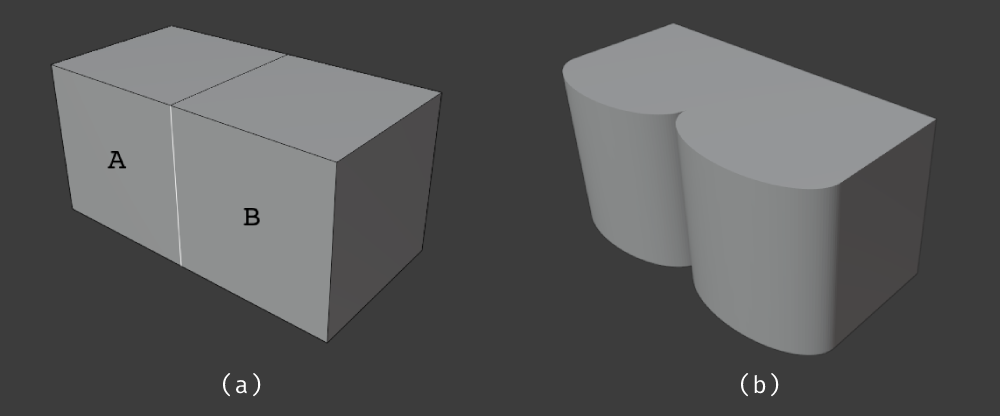
\includegraphics[width=15cm]{figuras/limitacao_solucao.png}
	}
	{\Fonte{Próprio autor}}	
\end{figure}

Na implementação atual, também não é realizada uma representação da região arredondada na árvore de formas. Isto ocorre devido ao fato dos índices dos diversos segmentos criados após a operação \texttt{roundShape} não seguirem um padrão específico de numeração, o que dificulta a recuperação da referência dos respectivos polígonos para armazenamento.

\section{Considerações finais}
\label{sec:consideracoes_capitulo_5}

Este capítulo descreveu as principais características da solução proposta, desde detalhes de implementação até algumas limitações encontradas. Por meio dos modelos gerados, percebe-se que a operação de deformação introduzida é capaz de produzir resultados interessantes, com estruturas arquitetônicas arredondadas que remetem a edifícios do mundo real. Assim, no próximo capítulo, serão apresentadas as conclusões finais da presente pesquisa.